\documentclass{beamer}
\usepackage[french]{babel} 
\usepackage[utf8]{inputenc} 
\usepackage[T1]{fontenc} 
\usepackage{graphicx}
\usepackage[utf8]{inputenc}
\usepackage{sectsty}
\usepackage{fancyhdr}
\usepackage{geometry}
\usepackage{tabularx,tabulary}

\title{3I013 Reunion du 8 Mars 2019}
\author{FM, DK, MF, NC}

%ce theme est le plus clean de Beamer le truc a ne pas utiliser c'est 'Warsaw'
\usetheme{default}

\addtobeamertemplate{footline}{
	\begin{flushright}
	\insertframenumber/\inserttotalframenumber
	\end{flushright}}

%debut des slides
\begin{document}


	%premiere diapo
	\begin{frame}
		\begin{center}
		\maketitle
		Ceci est la première diapo !\\
		\end{center}
	\end{frame}
	
	
	
	\begin{frame}
		\section{}
		\begin{flushleft}
		\frametitle{Sommaire}
		\tableofcontents{}
		\end{flushleft}
	\end{frame}
	
	
	\begin{frame}
	\section{Slide 2}
		\begin{center}
		\frametitle{Slide 2 : Objectif}
		\subsection{Objectif}
        \framesubtitle{L'expression des besoins}
		   Faire effectuer à un drone Bebop 2 une ronde en suivant un itinéraire prédéfini, et récupérer le retour vidéo en temps réel sur un iPod (qui pourra être placé dans un masque FPV).
		\end{center}
	\end{frame}
	
	\begin{frame}
	\section{Slide 3}
		\begin{center}
		\frametitle{Slide 3 : Besoins fonctionnels}
		\subsection{Besoins fonctionnels}
        \framesubtitle{L'expression des besoins}
		\begin{itemize}
		    \item Créer un plan de vol sur une carte, en spécifiant des points de passage pour former l'itinéraire ainsi que l'altitude du drone à ces points.
		    \item Communiquer le plan de vol au drone
		    \item Selectionner le plan de vol à exécuter
		    \item Lancer l'exécution du plan de vol
		    \item Bénéficier du retour vidéo dans l'iPod
		\end{itemize}
		\end{center}
	\end{frame}
	
	\begin{frame}
	\section{Slide 4}
		\begin{center}
		\frametitle{Slide 4 : Use Case}
		\subsection{Use Case}
        \framesubtitle{L'expression des besoins}
        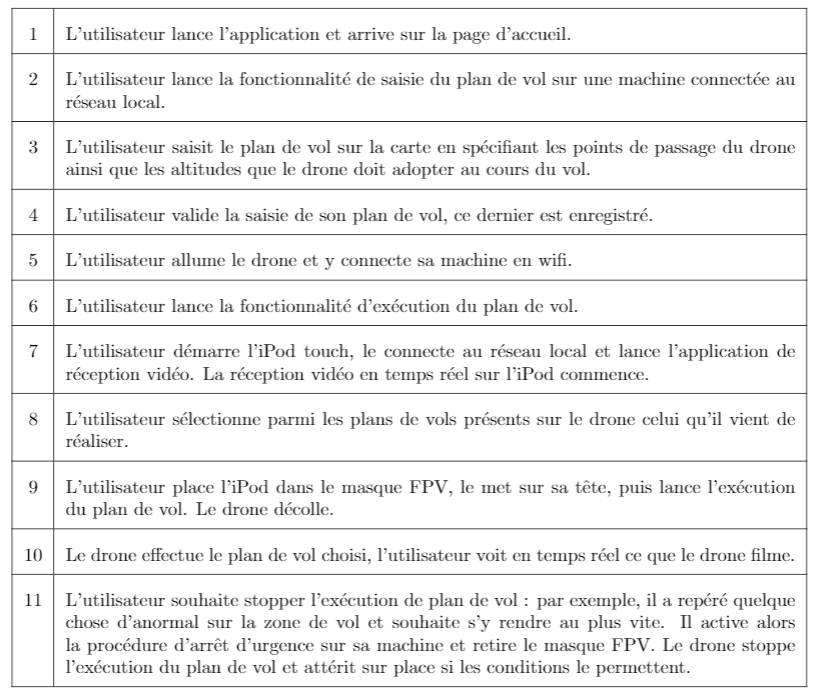
\includegraphics[scale=0.5]{Use_Case.PNG}
       \end{center}
	\end{frame}
	
	\begin{frame}
	\section{Slide 5}
		\begin{center}
		\frametitle{Slide 5 : Solutions étudiées}
		\subsection{Solutions étudiées}
        \framesubtitle{Les solutions}
            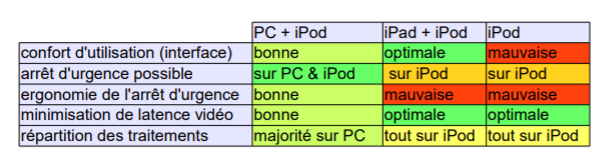
\includegraphics[scale=0.9]{comparatif.PNG}
		\end{center}
	\end{frame}
	
		
	\begin{frame}
	\section{Slide 6}
		\begin{center}
		\frametitle{Slide 6 : Solution retenue}
		\subsection{Solution retenue}
        \framesubtitle{Les solutions}
            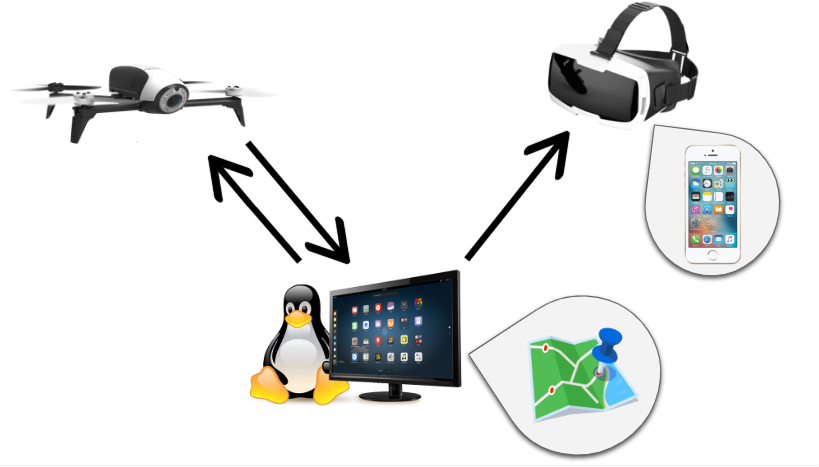
\includegraphics[scale=0.65]{shcema_archi.png}
		\end{center}
	\end{frame}
	
	\begin{frame}
	\section{Slide 7}
		\begin{center}
		\frametitle{Slide 7 : Contraintes}
		\subsection{Contraintes}
        \framesubtitle{Les solutions}
            \begin{itemize}
                \item Matériel : Bebop2, PC, iPod
                \item Un réseau local connecté au PC et à l'iPod, et bénéficiant d'un accès internet (API carte)
                \item Saisie du plan de vol ergonomique, simple, intuitive
                \item Arrêt d'urgence depuis le PC
            \end{itemize}
		\end{center}
	\end{frame}

	
\end{document}
